% Name: Load balancer
% Description: Clients reaching three identical application servers through a load balancer, with the servers sharing one database.
% Tags: load balancer, client-server, scalability, web architecture

\usetikzlibrary{arrows.meta, shapes.geometric}

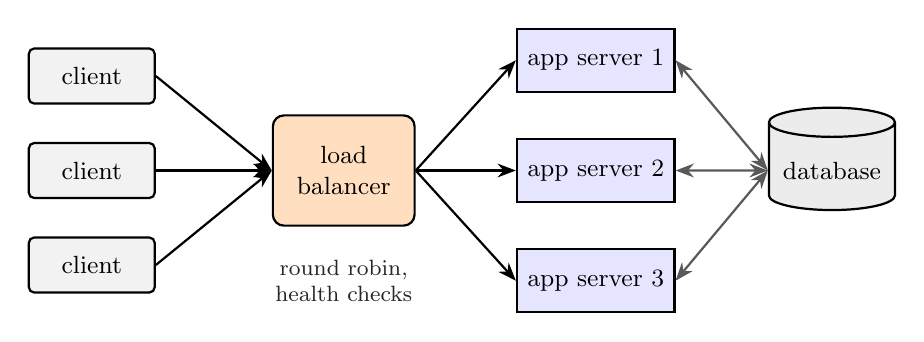
\begin{tikzpicture}[>={Stealth}, thick, every node/.style={font=\small},
    client/.style={draw, fill=gray!10, rounded corners=2pt, minimum width=16mm, minimum height=7mm},
    server/.style={draw, fill=blue!10, minimum width=20mm, minimum height=8mm}]
  \foreach \i/\y in {1/1.2, 2/0, 3/-1.2} \node[client] (c\i) at (0,\y) {client};
  \node[draw, fill=orange!25, rounded corners, minimum width=18mm, minimum height=14mm, align=center] (lb) at (3.2,0) {load\\balancer};
  \foreach \i/\y in {1/1.4, 2/0, 3/-1.4} \node[server] (s\i) at (6.4,\y) {app server \i};
  \node[draw, cylinder, shape border rotate=90, aspect=0.25, fill=gray!15, minimum width=16mm, minimum height=13mm] (db) at (9.4,0) {database};
  \foreach \i in {1,2,3} {
    \draw[->] (c\i.east) -- (lb.west);
    \draw[->] (lb.east) -- (s\i.west);
    \draw[<->, gray!70!black] (s\i.east) -- (db.west);
  }
  \node[font=\footnotesize, align=center, gray!30!black] at (3.2,-1.4) {round robin,\\health checks};
\end{tikzpicture}
